%
% laserAufweiten.tex -- Bild zum Thema Optische Fouriertransformation <opt>
%
% (c) 2023 Marco Niederberger, Yanick Schoch; OST Ostschweizer Fachhochschule
%

\documentclass[tikz]{standalone}
\usepackage{txfonts}
\usepackage{pgfplots}

\pgfplotsset{compat=1.16}
\def\skala{1}

\usetikzlibrary{arrows,intersections,math}
\usetikzlibrary{decorations.markings, calc}

%% Lense (x, height, curvature)
\newcommand{\lense}[3]{
    \def\curvature{0.2}
    \path[fill=glass, draw=black, line width = 0.6, opacity=0.8] (#1,-#2) .. controls (#1 - #3,0) .. (#1,#2) .. controls (#1 + #3,0) .. (#1,-#2);
}

%% Axis (x, textAbove, textBelow)
\newcommand{\xAxis}[3]{%
    \def\lenseX{2.5}
    \draw[->, thin] (#1,-\lenseX)--(#1,\lenseX) node[above]{#2};
    \node[] at (#1, -\lenseX - 0.5){#3};
}

%% Dimension arrow (xStart, xEnd)
\newcommand{\dimensionBetweenLenses}[3]{%
    \def\dimensionHeight{-2.3}
    \draw[<->] (#1, \dimensionHeight)--(#2, \dimensionHeight) node[above,midway] {#3};
}

% Styles
%% Arrow in the Middle
\tikzset{arrow inside/.style = {postaction=decorate,decoration={markings,mark=at position 0.52 with \arrow{stealth}}}}

% Define Color
\definecolor{glass}{cmyk}{0.2,0,0,0}

\begin{document}

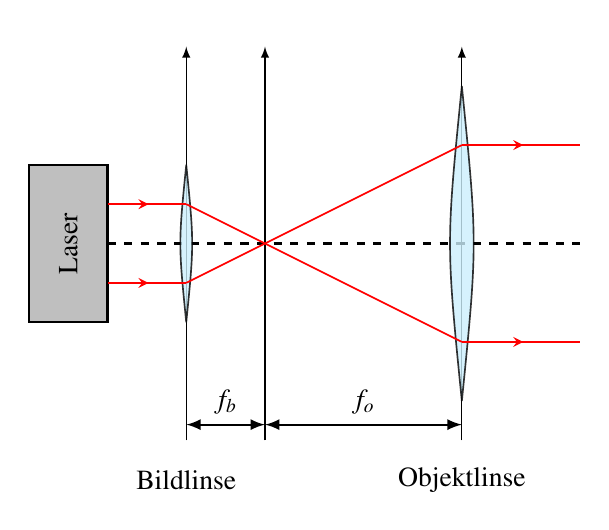
\begin{tikzpicture}[>=latex,thick,scale=\skala]

    % xAxis
    \xAxis{-1}{}{Bildlinse}
    \xAxis{0}{}{}
    \xAxis{2.5}{}{Objektlinse}

    % Optical plane
    \draw[dashed] (-2,0)--(4,0);

    \dimensionBetweenLenses{-1}{0}{$f_b$}
    \dimensionBetweenLenses{0}{2.5}{$f_o$}

    % Laser
    \draw[fill=lightgray] (-3, -1) rectangle (-2, 1) node[rotate=90, pos=0.5] {Laser};

    % Lenses
    \lense{-1}{1}{.1}
    \lense{2.5}{2}{.2}

    % Rays
    \draw[red, line width = 0.6, arrow inside] (-2, 0.5) -- (-1, 0.5);
    \draw[red, line width = 0.6, arrow inside] (-2, -0.5) -- (-1, -0.5);

    \draw[red, line width = 0.6, arrow inside] (2.5, 1.25) -- (4, 1.25);
    \draw[red, line width = 0.6, arrow inside] (2.5, -1.25) -- (4, -1.25);

    \draw[red, line width = 0.6] (-1, 0.5) -- (2.5, -1.25);
    \draw[red, line width = 0.6] (-1, -0.5) -- (2.5, 1.25);

\end{tikzpicture}
\end{document}

